\documentclass[margin=5mm]{standalone}
\usepackage[dvipsnames]{xcolor}
\usepackage{pgfplots}
\usepackage{tikz}
\usepackage[tikz]{ocgx2}

\pgfplotsset{compat=1.18}
\begin{document}

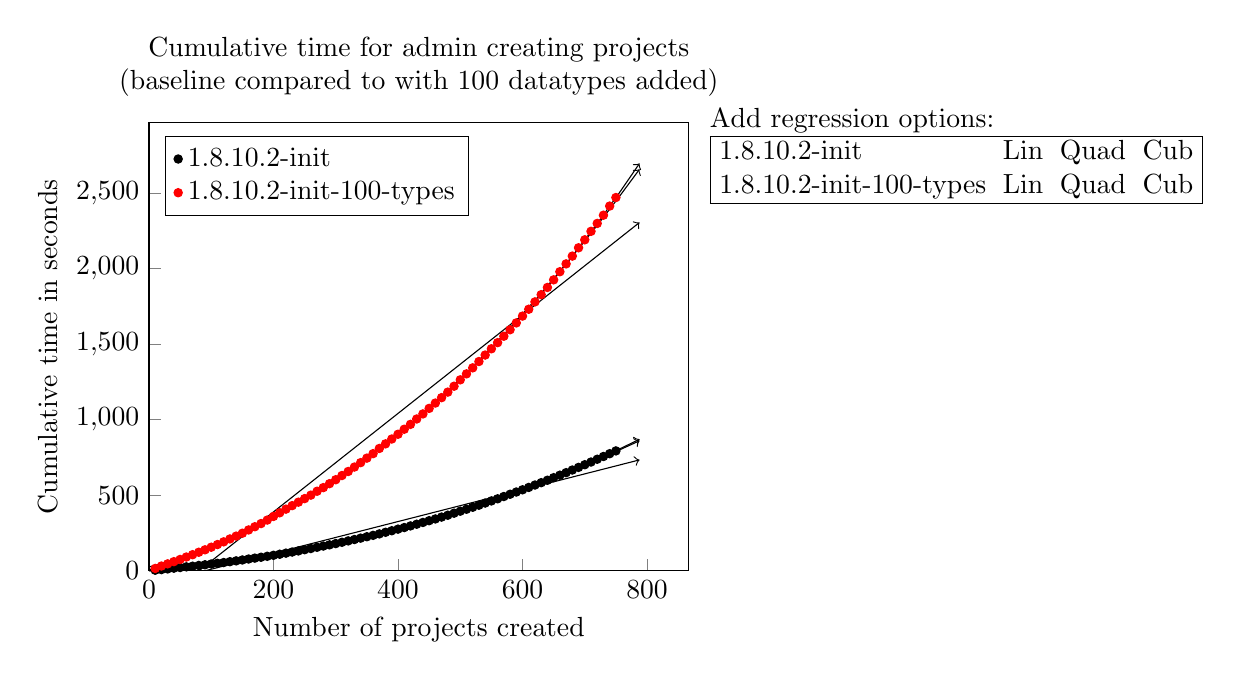
\begin{tikzpicture}
    \begin{axis}[
        align = center,
        legend pos = north west,
        legend cell align = left,
        xlabel = Number of projects created,
        ylabel = Cumulative time in seconds,
        xtick pos = left,
        ytick pos = left,
        scaled ticks = false,
        xmin = 0,
        ymin = 0,
        title = {Cumulative time for admin creating projects (baseline compared to with 100 datatypes added)},
        title style = {text width = 0.8\textwidth},
        legend entries={\switchocg{1.8.10.2-init}{1.8.10.2-init},\switchocg{1.8.10.2-init-100-types}{1.8.10.2-init-100-types}}]
        \begin{scope}[ocg = {ref = 1.8.10.2-init-Lin, status = invisible}]
            \plot[domain=0:788,->,forget plot] (\x,{-93.723738018017996864728047512471675872802734375 + 1.0511333456614508907733807063777931034564971923828125*(\x)^1});
        \end{scope}
        \begin{scope}[ocg = {ref = 1.8.10.2-init-Quad, status = invisible}]
            \plot[domain=0:788,->,forget plot] (\x,{9.464285849685136753350889193825423717498779296875 + 0.2470708220170104441049119259332655929028987884521484375*(\x)^1 + 0.00105797700479531679718103731602241168729960918426513671875*(\x)^2});
        \end{scope}
        \begin{scope}[ocg = {ref = 1.8.10.2-init-Cub, status = invisible}]
            \plot[domain=0:788,->,forget plot] (\x,{2.788357353243510861062759431661106646060943603515625 + 0.349116338573639495290734657828579656779766082763671875*(\x)^1 + 0.000724514042935094277654572980651437319465912878513336181640625*(\x)^2 + 0.0000002925113700528269138011173110258678065065396367572247982025146484375*(\x)^3});
        \end{scope}
        \begin{scope}[ocg = {ref = 1.8.10.2-init, status = visible}]
            \addplot[
                only marks,
                color = black,
                mark = *,
                mark size = 1.5 pt
            ]coordinates {(10,4.887)(20,8.825)(30,13.367)(40,18.302)(50,22.581)(60,27.105)(70,31.225)(80,36.253)(90,40.699)(100,45.826)(110,50.619)(120,55.553)(130,61.14)(140,66.599)(150,72.476)(160,78.857)(170,84.783)(180,90.605)(190,96.932)(200,103.539)(210,110.453)(220,117.712)(230,124.937)(240,132.344)(250,140.433)(260,148.274)(270,156.544)(280,164.592)(290,172.613)(300,180.944)(310,189.581)(320,198.722)(330,207.813)(340,217.042)(350,226.233)(360,235.47)(370,245.083)(380,255.682)(390,266.019)(400,276.529)(410,287.009)(420,297.771)(430,309.042)(440,320.68)(450,332.334)(460,343.9)(470,356.336)(480,368.683)(490,381.941)(500,395.275)(510,408.153)(520,421.309)(530,434.891)(540,449.083)(550,463.145)(560,477.218)(570,492.225)(580,507.293)(590,522.037)(600,536.813)(610,552.411)(620,568.334)(630,583.783)(640,599.932)(650,616.882)(660,633.313)(670,650.114)(680,667.53)(690,684.981)(700,702.645)(710,720.424)(720,738.801)(730,757.017)(740,775.532)(750,793.99)};
        \end{scope}
        \begin{scope}[ocg = {ref = 1.8.10.2-init-100-types-Lin, status = invisible}]
            \plot[domain=0:788,->,forget plot] (\x,{-260.67619135135117858226294629275798797607421875 + 3.256414819345660571769940361264161765575408935546875*(\x)^1});
        \end{scope}
        \begin{scope}[ocg = {ref = 1.8.10.2-init-100-types-Quad, status = invisible}]
            \plot[domain=0:788,->,forget plot] (\x,{26.24828913735615998348293942399322986602783203125 + 1.020639646706381409302366591873578727245330810546875*(\x)^1 + 0.00294180943768326298715098943148404941894114017486572265625*(\x)^2});
        \end{scope}
        \begin{scope}[ocg = {ref = 1.8.10.2-init-100-types-Cub, status = invisible}]
            \plot[domain=0:788,->,forget plot] (\x,{-0.184545581472180530990812030722736380994319915771484375 + 1.4246811630851989871615614902111701667308807373046875*(\x)^1 + 0.0016214880231563669372996105977335901116020977497100830078125*(\x)^2 + 0.000001158176679409558411764356346262960784088136279024183750152587890625*(\x)^3});
        \end{scope}
        \begin{scope}[ocg = {ref = 1.8.10.2-init-100-types, status = visible}]
            \addplot[
                only marks,
                color = red,
                mark = *,
                mark size = 1.5 pt
            ]coordinates {(10,16.512)(20,32.474)(30,46.817)(40,61.427)(50,75.999)(60,92.058)(70,107.382)(80,123.673)(90,139.787)(100,156.898)(110,174.58)(120,192.488)(130,211.55)(140,230.345)(150,249.393)(160,271.058)(170,292.395)(180,313.38)(190,336.521)(200,360.628)(210,384.814)(220,408.851)(230,432.07)(240,454.959)(250,478.353)(260,501.424)(270,527.2)(280,551.181)(290,577.294)(300,603.426)(310,631.23)(320,657.891)(330,687.255)(340,716.416)(350,746.224)(360,775.949)(370,810.206)(380,840.765)(390,872.673)(400,904.154)(410,937.208)(420,969.515)(430,1005.065)(440,1038.704)(450,1075.273)(460,1110.589)(470,1146.281)(480,1182.891)(490,1221.907)(500,1264.154)(510,1303.752)(520,1343.413)(530,1385.269)(540,1428.156)(550,1469.588)(560,1510.125)(570,1552.632)(580,1595.431)(590,1640.717)(600,1685.825)(610,1731.074)(620,1779.767)(630,1827.599)(640,1875.292)(650,1925.581)(660,1979.361)(670,2031.191)(680,2082.614)(690,2137.681)(700,2190.463)(710,2246.492)(720,2298.797)(730,2353.247)(740,2413.621)(750,2470.133)};
        \end{scope}
    \end{axis}
    \begin{scope}
        \addtolength{\tabcolsep}{-0.3em}
        \node [below right, shape=rectangle, align=left](regressiontable) at (7,6) {
            Add regression options: \\
            \begin{tabular}{|llll|}
                \hline
                1.8.10.2-init & \switchocg{1.8.10.2-init-Lin}{Lin} & \switchocg{1.8.10.2-init-Quad}{Quad} & \switchocg{1.8.10.2-init-Cub}{Cub} \\
                1.8.10.2-init-100-types & \switchocg{1.8.10.2-init-100-types-Lin}{Lin} & \switchocg{1.8.10.2-init-100-types-Quad}{Quad} & \switchocg{1.8.10.2-init-100-types-Cub}{Cub} \\
                \hline
            \end{tabular}
        };
    \end{scope}
\end{tikzpicture}

\end{document}